
\documentclass[a4paper, 12pt, twoside]{book}

%% Escrevendo em portugues:
\usepackage[brazil]{babel}	
\usepackage[T1]{fontenc}
\usepackage{float}
\usepackage[scaled]{helvet}
\usepackage[utf8]{inputenc}
\usepackage{upquote} %fix minted quotes
\usepackage{parskip} %fix paragraph spacing inside tubainabox
\usepackage{setspace}
\usepackage{monografia}
\usepackage{hyperref}
\usepackage[a4paper, top=46mm, left=29mm, right=29mm, bottom=32mm, includefoot]{geometry}

\usepackage[pdftex]{graphicx}           % usamos arquivos pdf/png como figuras

\usepackage{fancyhdr}

\raggedbottom

\newcommand{\codechunk}[1]{{\ttfamily {\small #1}}}



\begin{document}

\begin{titlepage}
\vspace*{\fill}
\vspace{-5cm}
\center{\begin{spacing}{1.0}\huge \textbf{\textsc{MetricMiner: uma ferramenta web de apoio à mineração de repositórios de software}}\end{spacing}}
\vspace{2cm}
\center\textsc{{\Large Francisco Sokol}}
\vspace{1cm}
\center\textsc{{\large Orientador: Marco Aurélio Gerosa}}
\center\textsc{{\large Co-orientador: Mauricio Finavaro Aniche}}
\vfill
\end{titlepage}

% \title{MetricMiner: uma ferramenta web de apoio à mineração de repositórios de software}
% \author{Francisco Sokol}
% \maketitle

\pagestyle{plain}

\pagenumbering{arabic}
\setcounter{page}{1}

\tableofcontents

\newpage

\chapter{Introdução}

    Evolução de Software é uma área da Engenharia de Software que estuda as atividades de
    desenvolvimento em um sistema de software após a sua concepção inicial e implantação em
    produção. Esse termo foi usado pela primeira vez em um trabalho publicado por Manny 
    Lehman \cite{DBLP:series/springer/Mens08}. Neste trabalho, o autor enuncia as 
    ``leis da evolução de software'', defendendo que programas que representam alguma atividade
    do mundo real evoluem continuamente, caso contrário, se tornam menos úteis e perdem seu 
    valor \cite{Lehman1980b}. Além disso, Lehman afirma que este processo de mudança contínua
    faz com que a complexidade do software cresça inevitavelmente, tornando sua estrutura
    cada vez mais pobre e seu custo de manutenção maior.
    
    Considerando ainda diversos trabalhos indicando que o custo de manutenção de um software 
    ultrapassa 50\% do custo total de um projeto, observa-se que encontrar meios de se
    manter a qualidade interna de um software é importante. Por meio do desenvolvimento 
    ferramentas e métodos, a evolução de software busca entender e controlar esse processo
    para o tornar mais eficiente.
    
    Nesse contexto, a Mineração de Repositórios de Software estuda esse processo de evolução 
    de forma empírica, por meio da análise dos artefatos envolvidos no seu desenvolvimento 
    como código fonte, dados do sistema de controle de versão e sistemas de rastreamento 
    de bugs \cite{Kagdi:2007}. Por meio da mineração desses dados, podem ser extraídas diversas
    informações úteis ao desenvolvimento de um software, como por exemplo a indentificação de classes que são 
    modificadas constantemente, classes mais propensas a falhas, entre outras. Com essas informações, 
    equipes de desenvolvimento podem tomar ações para aprimorar o processo de desenvolvimento 
    do sistema.

    \section{Motivação}
        Para desenvolver um trabalho em mineração de repositórios, o pesquisador é obrigado 
        a carregar diversos projetos em sua estação de trabalho e realizar uma série de cálculos
        sobre o código dos projetos e sobre os metadados de seu repositório. Esse processo 
        requer a instalação de diversas ferramentas e bibliotecas localmente para reaproveitar
        as ferramentas desenvolvidas nessa área, tornando o processo trabalhoso e demorado.

        Além de ser um processo complexo, esse tipo de pesquisa consome muitos 
        recursos computacionais. Baixar os repositórios a serem minerados consome um volume
        considerável de banda. Depois, os dados devem ser processados e persistidos em um 
        banco de dados, ocupando um grande volume de disco. Só então o pesquisador pode 
        calcular métricas sobre esses dados, além de extrair relações entre os metadados do 
        histórico do sistema de controle de versão, gastando uma quantidade grande de
        processamento de CPU. Só depois de passar por todas essas etapas, é possível extrair
        dados e avaliar hipóteses por meio de análises estatísticas.

        Dessas dificuldades surgiu a motivação para o desenvolvimento do MetricMiner,
        uma aplicação web que realiza todas as etapas da mineração de um repositório de 
        software. Essa ferramenta disponibiliza um grande volume de dados já processados 
        prontos para serem extraídos e analisados pelo pesquisador, poupando tempo e recursos 
        computacionais.
    
    \section{Estrutura da monografia}
        Este trabalho está estruturado da seguinte forma: 
        \begin{itemize}
            \item Seção \ref{ch:conceitos}: nesta seção são abordados temas 
                envolvidos no desenvolvimento desse trabalho, em um breve levantamento bibliográfico.
            \item Seção \ref{ch:arquitetura}: apresenta a arquitetura e as tecnologias
            envolvidas no desenvolvimento do MetricMiner.
            \item Seção \ref{ch:avaliacao}: expõe os resultados obtidos com a ferramenta 
                na mineração de repositórios de projetos de código aberto.
            \item Seção \ref{ch:conclusao}: análise dos resultados e levantamento 
                de possíveis extensões futuras do projeto.
            \item Seção \ref{ch:subjetiva}: apresenta as impressões do aluno na realização 
                desse trabalho e a sua relação com o curso de Bacharelado em Ciência da Computação.
        \end{itemize}
    
\chapter{Mineração de Repositórios de Software} \label{ch:conceitos}
    Esta seção é uma introdução aos principais temas de pesquisa envolvidos no desenvolvimento
    deste trabalho. As subseções \ref{sc:evolucao} e \ref{sc:mineracao} contém, respectivamente, 
    uma introdução a Evolução de Software e Mineração de Repositórios de Software, as duas áreas 
    da Engenharia de Software envolvidas no desenvolvimento desse trabalho. Na subceção 
    \ref{sc:metricas}, são apresentadas algumas métricas de código fonte implementadas no 
    MetricMiner. A subseção \ref{ch:trabalhos}, contém uma breve análise de outras ferramentas
    relacionadas ao MetricMiner e à área de mineração de repositórios de software.

    \section{Evolução de software} \label{sc:evolucao}
        No final da década de sessenta, o termo ``manutenção de software'' foi definido 
        como qualquer atividade de desenvolvimento realizada sobre o software após a sua
        entrega e implantação inicial. Essa também era a visão estabelecida no modelo de
        desenvolvimento de software em cascata, proposto por Royce, em 1970 
        \cite{DBLP:series/springer/Mens08}. Neste modelo, a manutenção do sistema era a fase final do 
        desenvolvimento, em que eram feitos apenas pequenos ajustes e correção de erros.
        
        Com o passar do tempo, percebeu-se que esse processo era pouco eficiente, 
        principalmente porque os requisitos levantados apenas na fase inicial do projeto se 
        modificavam frequentemente, mesmo durante a fase de manutenção. Na tentativa de compreender
        a natureza dessas mudanças no processo de desenvolvimento, Manny Lehman realizou diversos 
        estudos empíricos sobre o desenvolvimento de sistemas da IBM \textbf{colocar refs aqui} 
        (ver nom\cite{DBLP:series/springer/Mens08})
        
        No trabalho publicado em \cite{Lehman1980b}, Lehman define três classes de programas.
        A classe S, contém programas cujas funcionalidades podem ser especificadas formalmente e possuem uma 
        solução precisa. Problemas famosos como o do caixeiro viajante, n-rainhas, fluxo máximo, entre outros,
        são exemplos que podem servir de especificação para um programa da classe S. Esse 
        tipo de programa é estático (a letra S vem de \textit{static}) pois, uma vez estabelecida a 
        solução para seu problema, esta satisfaz seus requisitos por completo.
        
        A classe P, contém programas criados para solucionar algum problema do mundo real, que também  pode ser 
        especificado formalmente, porém não pode ser solucionado com precisão absoluta (a letra P 
        vem de \textit{real world \textbf{p}roblem solution}). Exemplos
        dessa classe incluem programas para previsão do tempo, um jogador de xadrez, um 
        escalonador de vôos e linhas de trem, entre outros. Os resultados obtidos por programas dessa
        classe não são soluções exatas do problema, devido a complexidade ou a própria natureza deste.
        Programas da classe P, portanto, também possuem seus requisitos especificados com precisão e 
        as mudanças realizadas sobre eles acontecem apenas com o objetivo de aprimorar sua performance ou a qualidade dos resultados.
        
        Os programas da classe E são aqueles cuja a especificação não pode ser definida completamente.
        Tais programas são inseridos no mundo real para agilizar tarefas de seu domínio, modificando 
        a forma como as atividades são realizadas. Exemplos de programas da classe E são: sistemas 
        operacionais, sistemas de controle aéreo, de mercado financeiro, entre outros. Programas 
        dessa classe modificam o seu domínio de aplicação após sua implantação inicial, então é 
        natural que com o passar do tempo novos requisitos sejam levantados para satisfazer 
        novas necessidades da atividade que foi alterada. Programas dessa classe estão
        sujeitos a sofrerem alterações constantes após a implantação inicial e, portanto estão
        em um processo de evolução constante (a letra E vem de \textit{evolution}).
        
        Assim, sistemas da classe E estão mais sujeitos a mudanças do que programas das classes S 
        e P, por isso Lehman dirigiu seu trabalho sobre a análise da evolução de programas da 
        classe E. Em uma tentativa de descrever esse processo de evolução em \cite{Lehman1980b}, o 
        autor propõe as \textit{leis da evolução de software}:
        \begin{itemize}
            \item Mudança contínua: Um programa da classe E muda continuamente, caso contrário, se 
                   torna menos útil gradativamente.
            \item Complexidade crescente: Com o processo de mudança contínua, a complexidade do 
                  software cresce, a menos que sejam dirigidos esforços para reduzir ou manter essa 
                  complexidade.
            \item Auto regulação: A evolução de software é um processo auto regulado pelo \textit{feedback} 
                  das mudanças feitas no sistema e as reações a essas mudanças no domínio em que ele 
                  é utilizado.
            \item Conservação de estabilidade organizacional: A taxa com que as modificações são 
                  feitas sobre o software ao longo de seu ciclo de vida é estatisticamente invariante.
            \item Conservação de familiaridade: A evolução de um programa é limitada pela 
                  familiaridade com que seus desenvoldores tem com o sistema.
        \end{itemize}

        O trabalho de Lehman foi o primeiro a utilizar o termo ``evolução de software'' para
        descrever o processo de mudança sobre sistemas de software. Hoje, essa área de pesquisa
        envolve diversos temas, como: engenharia reversa e reengenharia, qualidade de software,
        gerenciamento de configuração de software, estimativas de custos, entre outros 
        \cite{DBLP:series/springer/Mens08}.
        
        Ainda não há um consenso da validade dessas leis para sistemas de software de código aberto. 
        Em  \cite{DBLP:series/springer/Fernandez-RamilLWC08}, os autores discutem a validade dessas
        leis analisando diversos estudos realizados sobre projetos de código aberto, concluindo que
        algumas das leis se aplicam, enquanto ainda não há evidências concretas de validade da 
        maioria delas.
        
    \section{Mineração de repositórios de software} \label{sc:mineracao}
        Compreender o processo de evolução de um software é uma tarefa complexa. Sistemas de software grandes possuem um longo histórico de desenvolvimento com diversos desenvolvedores trabalhando em diferentes partes do sistema. É comum que nenhum desenvolvedor conheça o código do sistema por completo por conta da sua complexidade ou mesmo porque os integrantes que iniciaram o desenvolvimento do projeto já não fazem mais parte da equipe. Portanto, analisar os dados históricos do desenvolvimento de um software grande manualmente é inviável. 

        Assim, a Mineração de Repositórios de Software analisa a evolução de software de forma automatizada aplicando técnicas da Mineração de Dados sobre o histórico do desenvolvimento de sistemas de software \cite{workshop-gustavo-aniche}. Os estudos desenvolvidos nessa área podem revelar informações úteis ao desenvolvimento de um projeto em particular ou ainda encontrar padrões na evolução de software que podem ser generalizados para outros sistemas (mas sempre com as limitações de um estudo empírico).

        O termo ``repositório de software'' abrange todos os artefatos produzidos durante o 
        desenvolvimento de um sistema de software, desde os arquivos com o código fonte do sistema que 
        podem estar armazenados em um sistema de controle de versão, até mensagens em listas de
        emails trocadas entre os desenvolvedores. Tais repositórios contém informações valiosas, 
        que podem ser exploradas para se compreender a evolução de software e contribuir com o 
        desenvolvimento do projeto.

        Em \cite{DBLP:series/springer/DAmbrosGLP08}, os autores destacam os seguintes tópicos 
        estudados na análise de repositórios de software:
        \begin{itemize}
            \item \textbf{Concentração do trabalho dos desenvolvedores e análise de redes sociais}. 
            O objetivo nesse tópico é descobrir quanto e em quais pontos do software os desenvolvedores estão dedicando mais seus esforços e como eles se comunicam entre si, para buscar soluções em problemas no processo de desenvolvimento e na estrutura da equipe.
            \item \textbf{Impacto e propagação de alterações}. 
            Busca ententer o efeito das mudanças feitas em
            certa parte do sistema sobre o resto do código do projeto. Compreendendo melhor o efeito
            dessas alterações, a equipe pode estimar melhor os custos de certa tarefa. Além disso,
            um desenvolvedor pode ser informado de quais arquivos ele precisará checar após ter feito
            uma certa alteração.
            \item \textbf{Análise de tendências e \textit{hotspots}}. 
            \textit{Hotspots} são pontos do software
            que sofrem alterações frequentemente. Encontrar tais pontos do sistema, pode ajudar a 
            levantar deficiências na arquitetura do projeto e sugerir possíveis refotatorações para
            aprimorar sua manutenabilidade.
            \item \textbf{Previsão de falhas e defeitos}.
            Os dados disponíveis em repositórios de software
            podem ser usados como entrada para algoritmos de aprendizagem de máquina, para criar
            modelos preditivos de possíveis falhas no sistema. Com esse modelo, a equipe pode
            tomar ações preventivas para previnir tais falhas em versões futuras.
        \end{itemize}

        Neste trabalho, os autores também descrevem um modelo de dados para armazenar informações do
        sistema de controle de versão e de um sistema de rastreamento de bugs de um certo software.
        Esse modelo guarda os dados de cada \textit{commit} do projeto, como arquivos modificados, linha adicionadas/removidas, mensagem do autor e associa essas informações com um bug extraído 
        do sistema de rastreamento de bugs. Para popular esse modelo, é utilizado arquivo de log
        do sistema de controle de versão \textit{CVS} e o sistema de rastreamento de bugs 
        \textit{Bugzilla}. Os autores denominaram esse modelo de dados \textit{Release History 
        Database} (RHDB). Com os dados deste modelo, foram desenvolvidas três ferramentas para 
        vizualização das informações extraídas.

        Em \cite{Kagdi:2007}, é apresentada uma avaliação de diversos trabalhos de Mineração
        de Repositórios de Software (MRS). A partir da análise desses trabalhos, os autores propõem
        uma taxonomia para classificar os estudos nessa área. Essa classificação se baseia
        em quatro aspectos dos estudos avaliados: a fonte de informação dos dados, os objetivos
        do trabalho, a metodologia adotada para analisar os dados e a granularidade dos dados
        analisados.

        Em relação às fontes de informação, três categorias foram levantadas: as versões do software 
        e de seus artefatos, as diferenças entre esses artefatos e os metadados de cada mudança
        feita sobre o software. As versões e alterações do software podem ser coletadas de Sistemas
        de Controle de Versão (SCV). Os metadados dessas alterações, como autor, data e comentário do 
        autor também podem ser extraídas do SCV e complementadas com dados de um sistema de 
        rastreamento de bugs e mensagens trocadas pelos desenvolvedores em listas de email.

        Quanto aos objetivos dos estudos em MRS, os autores classificam os trabalhos analisados
        em relação às questões de pesquisa que dirigem esses estudos. Foram definidas duas classes
        de questão de pesquisa. A primeira é composta por questões do tipo \textit{market-basket}
        (termo emprestado da mineração de dados). São estudos que buscam avaliar a relação
        entre certos eventos e dados da evolução de software. Questões de pesquisa como ``se um evento A
        acontece quais outros eventos decorrem de A?'' se enquadram nesse conjunto. A segunda classe
        é composta por questões de predomínio (\textit{prevalence question}). Questões como ``quantas
        vezes um determinado módulo foi modificado?'' ou ``quais classes foram reutilizadas no sistema?''
        são exemplos de questões dessa classe.

        Dois métodos principais foram encontrados nos estudos avaliados. O primeiro é o estudo
        de mudanças sobre propriedades do software (\textit{changes to properties}), que é a 
        análise de propriedades de alto nível dos sistemas, como métricas de complexidade ou
        manutenabilidade, por exemplo. Na segunda estratégia de estudo, são analisadas 
        as alterações diretamente nos artefatos, em um nível mais baixo 
        (\textit{changes to artifacts}).

    \section{Métricas de código} \label{sc:metricas}

    % Explique as principais que usamos no MetricMiner, ok? Complexidade ciclomática, Acoplamento aferente e eferente, LCOM, Linhas de código por método.

\chapter{Trabalhos relacionados} \label{ch:trabalhos}

(revisar)
% As ferramentas que vc citou ajudam a calcular métricas de código, mas não olham muito evolução de software, certo (tirando o sonar)?
% Divida seus trabalhos relacionados em 2. Ferramentas de métrica de código, e ferramenta de MSR.
% Comente da Evoltrack, Oceano (do pessoal da UFF), CodeCity. Googla tb pelo professor Harald Gall, acha o site do grupo de pesquisa dele, lá tem as ferramentas dele, e vale a pena comentar.
% Faça também uma seção de "comparação". E mostre o que elas não tem e quais  são os principais problemas dela e pq fizemos o metricminer.

Nesta seção serão apresentadas ferramentas que se relacionam ao MetricMiner.
\section{Sonar}
    Não se conhece ferramentas web de suporte a mineração de repositórios de software. Uma ferramenta que se assemelha ao MetricMiner, é o Sonar \footnote{http://www.sonarsource.org/}, uma aplicação web que analisa o código fonte e extrai uma variedade de relatórios sobre o sistema, como resultados de métricas de código e dependências estruturais entre as classes. O foco desta ferramenta é apoiar a equipe de desenvolvimento e acompanhar a qualidade do código escrito. O Sonar não armazena metadados do sistema de controle versão e não permite que se extraia dados dos projetos armazenados, mas fornece uma interface de vizualização com muitos recursos. Por esses motivo, o Sonar é muito utilizado na indústria e pouco utilizado para fins acadêmicos.
    
    Diferentemente do Sonar, o MetricMiner tem o foco na área acadêmica, possibilitando que os usuários extraiam dados calculados pelo sistema para realizar a análise que desejar, sem focar tanto na vizualização dos dados armazenados.

\section{Eclipse Metrics}
    O Eclipse Metrics\footnote{http://metrics.sourceforge.net/} é um \textit{plugin} para o Eclipse que calcula uma variedade de métricas de código no ambiente do desenvolvedor. Dessa forma, para que se acompanhe a evolução do código do projeto é necessário executar manualmente o \textit{plugin} para os \textit{releases} que se deseja analisar. No MetricMiner, o cálculo das métricas é realizado sobre todo o histórico de versões do projeto analisado, sem que o usuário precise selecionar as versões manualmente. Além disso, não é necessário que o usuário configure nada em seu ambiente e nem que mantenha as versões que deseja analisar localmente.
    
\section{Kalibro}
    Desenvolvida no Brasil, o Kalibro\footnote{http://www.kalibro.org/} é uma ferramenta que calcula as principais métricas de código fonte. O foco do Kalibro é dar suporte ao desenvolvedor, sugerindo valores de referência para as métricas calculadas, apontando possíveis problemas no projeto analisado. A ferramenta permite que os valores de referência sejam configurados por projeto. Através de código JavaScript, é possível compor as métricas calculadas pelo Kalibro, permitindo que o usuário crie novas métricas. Assim como o Eclipse Metrics, o Kalibro não analisa todo o histório de versões, de forma que o usuário precisaria selecionar as versões e recalcular as métricas manualmente.
    
\chapter{MetricMiner} \label{ch:arquitetura}

    Todo o código e o histórico de desenvolvimento do MetricMiner se encontra hospedado no github: \url{http://github.com/metricminer/metricminer}. O MetricMiner surgiu a partir do rEvolution\footnote{http://github.com/mauricioaniche/rEvolution}, uma ferramenta de linha de comando que extrai dados de um repositório local e persiste em banco de dados  relacional. Boa parte do código do rEvolution pôde ser reutilizada no MetricMiner, como o componente que realiza a interface com o sistema de controle de versão, que será descrito com mais detalhes na seção \ref{sc:tecnologias}.

    As limitações do rEvolution serviram de motivação para o desenvolvimento do MetricMiner. Primeiramente, o rEvolution coleta dados de apenas único projeto, de forma que é necessário executar o programa manualmente para a mineração de sistemas diferentes. Além disso, a configuração para se executar o rEvolution é complexa. É necessário configurar a conexão com o banco de dados, instalar o sistema de controle de versão utilizado pelo projeto a ser minerado e carregar o projeto localmente (o que pode ser demorado dependendo do tamanho do projeto). 

    Assim, se decidiu que o MetricMiner deveria ser uma aplicação web, poupando o pesquisador de instalar e configurar qualquer ferramenta localmente. Além disso, sendo uma aplicação web, a ferramenta pode aproveitar a escalabilidade da computação em nuvem. Atualmente o MetricMiner está implantando sobre a infraestrutura de computação em nuvem da locaweb. Durante a fase de testes da ferramenta, a capacidade de armazenamento do disco chegou ao seu limite e foi necessário aumentar tal capacidade. Esse aprimoramento foi feito sem que fosse necessário reinstalar o servidor e sem que houvesse qualquer perda dos dados armazenados. O mesmo não seria possível se o MetricMiner não fosse uma aplicação web.

    Nas subçeções seguintes, o MetricMiner será descrito com maiores detalhes. Na subseção \ref{sc:tecnologias}, as tecnologias utilizadas para o desenvolvimento do sistema serão descritos brevemente. Em \ref{sc:abordagem}, será apresentado o fluxo do processo de mineração realizado pelo MetricMiner e as principais funcionalidades implementadas. Em \ref{sc:arquitetura}, serão presentados os detalhes da arquitetura da ferramenta.

    
    \section{Principais funcionalidades} \label{sc:abordagem}
        O MetricMiner possui uma interface web, pela qual os usuários podem cadastrar projetos de
        sofware para serem minerados. Para esse cadastro, devem ser fornecidos um nome e a url
        pública para o repositóriode código do projeto. Até o momento, os sistemas de controle de versão 
        suportados são o Git e o SVN.

        Como a maioria das etapas da mineração de dados são demoradas, como
        clonar repositórios, persistir suas informações no banco de dados e calcular métricas sobre o
        código fonte, essas tarefas são executadas de maneira assíncrona, por meio 
        de uma fila de execução representada no banco de dados. Cada tarefa é armazenada no sistema e 
        processada por um componente que constrói as dependências de cada tarefa e as executa na 
        ordem em que foram cadastradas.

        Portanto, após o cadastro do projeto, são registradas quatro tarefas relativas a esse 
        projeto: carregamento do repositório de código, processamento de todas as versões
        dos arquivos do repositório de seus metadados e armazenamento dos dados,
        remoção dos arquivos carregados e cálculo das métricas de código sobre todos
        as versões do código fonte do projeto.

        Ao final desse processo, todas as informações do projeto estão persistidas no banco de dados 
        e disponíveis para serem extraídas pelo pesquisador. É importante ressaltar que após a 
        extração dos dados do sistema de controle de versão, é possível implementar novas métricas 
        para serem calculadas sobre o código, sem precisar executar todos os passos anteriores 
        novamente. A Figura \ref{fig:diagrama} descreve as tarefas envolvidas no processo de 
        mineração sobre um repositório de software cadastrado na ferramenta.

        \begin{figure}[ht]
            \centering
            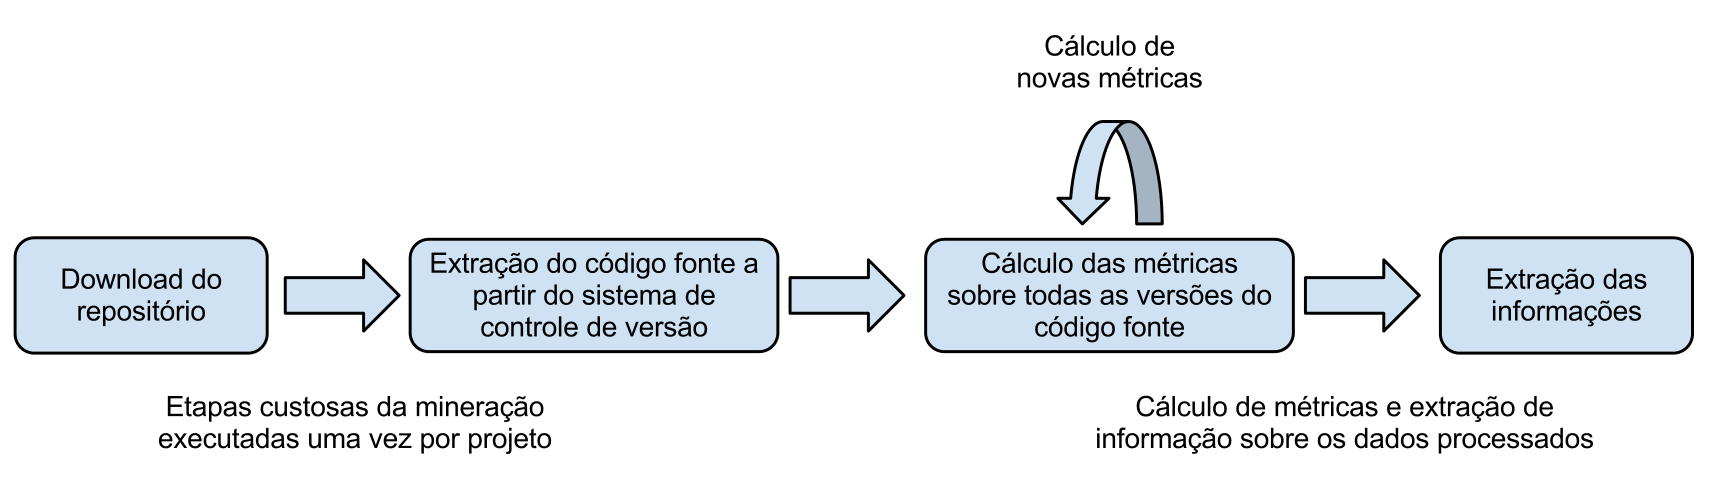
\includegraphics[width=1.0\textwidth]{img/diagrama.png}
            \caption{Diagrama do processo de mineração realizado pelo MetricMiner}
            \label{fig:diagrama}
        \end{figure}

        Cada projeto possui sua própria página no sistema. A Figura \ref{fig:screen_projeto} exibe a 
        tela de vizualização no MetricMiner do projeto Ant, software de código aberto da fundação     
        Apache com mais de doze mil \textit{commits}. Nessa tela, são exibidas informações básicas 
        sobre o projeto como número de \textit{commits}, número de \textit{commiters}, url do 
        repositório, data do primeiro e último \textit{commit}. São exibidos também dois gráficos 
        simples nos quais pode ser vizualizado o número de \textit{commits} nos últimos doze meses 
        (agrupados por mês) e o número de arquivos modificados em cada \textit{commit} nos últimos 
        seis meses (agrupados por \textit{commit}). Também podem ser adicionadas \textit{tags},
        para permitir que projetos de domínios semelhantes sejam agrupados.
    
        \begin{figure}[ht]
            \centering
            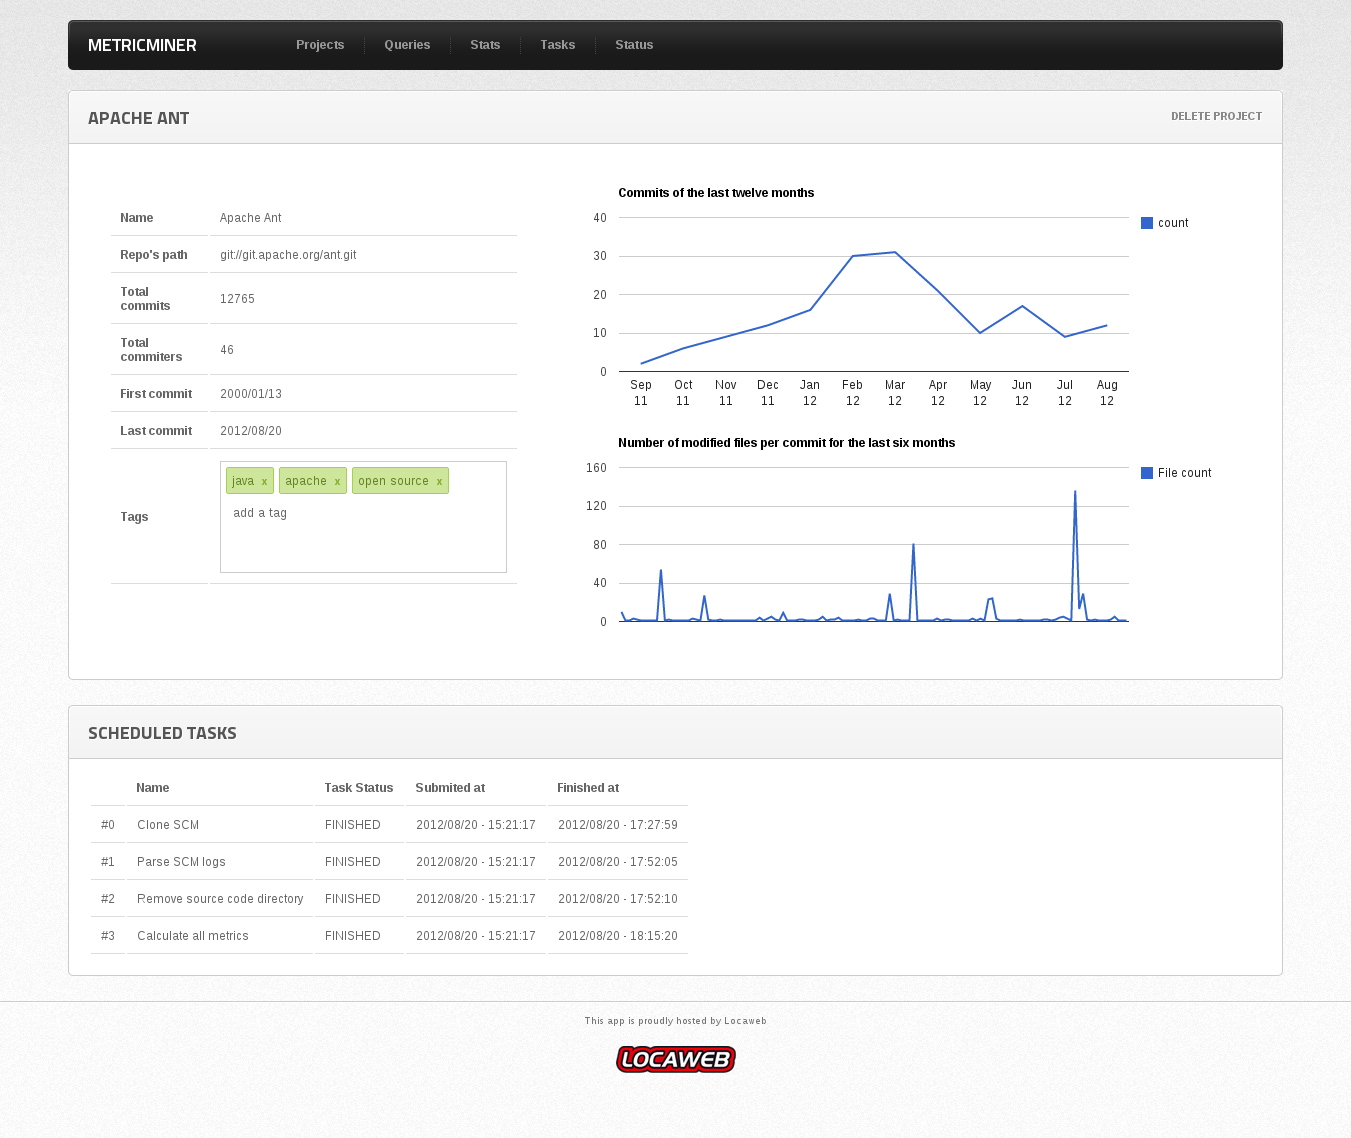
\includegraphics[width=1.00\textwidth]{img/ant.png}
            \caption{Tela de vizualização de projeto}
            \label{fig:screen_projeto}
        \end{figure}

        Após o fim do processamento do projeto, o usuário pode realizar consultas aos dados processados pela ferramenta. A Figura \ref{fig:screen_query} exibe a tela na qual é possível inserir uma consulta em SQL ao banco de dados do MetricMiner. Para preservarção da identidade, o nome e email dos autores são anonimizados, de forma que ao consultar o email de um desenvolvedor, por exemplo, é devolvido o resultado de uma função de hash do email desejado. Além disso, não é permitido realizar consultas sobre o código fonte dos projetos, dessa forma será possível minerar também sistemas de software da indústria, que não são distribuídos sob uma licença de código aberto.

        Depois de salvar a consulta, uma nova tarefa é adicionada à fila de execução e, ao final dessa tarefa, o usuário é informado por email do fim da execução da consulta e pode acessar a página da query para baixar os resultados em um arquivo no formato CSV (\textit{Comma Separated Values}). O usuário também pode acessar as queries criadas por outros usuários e reexecutar tais queries sobre a base de dados. Caso ocorra alguma falha na execução da query (um erro de sintaxe de SQL, por exemplo), a \textit{stacktrace} da falha é armazenada e o usuário pode visulizá-la na página de resultados.

        \begin{figure}[ht]
            \centering
            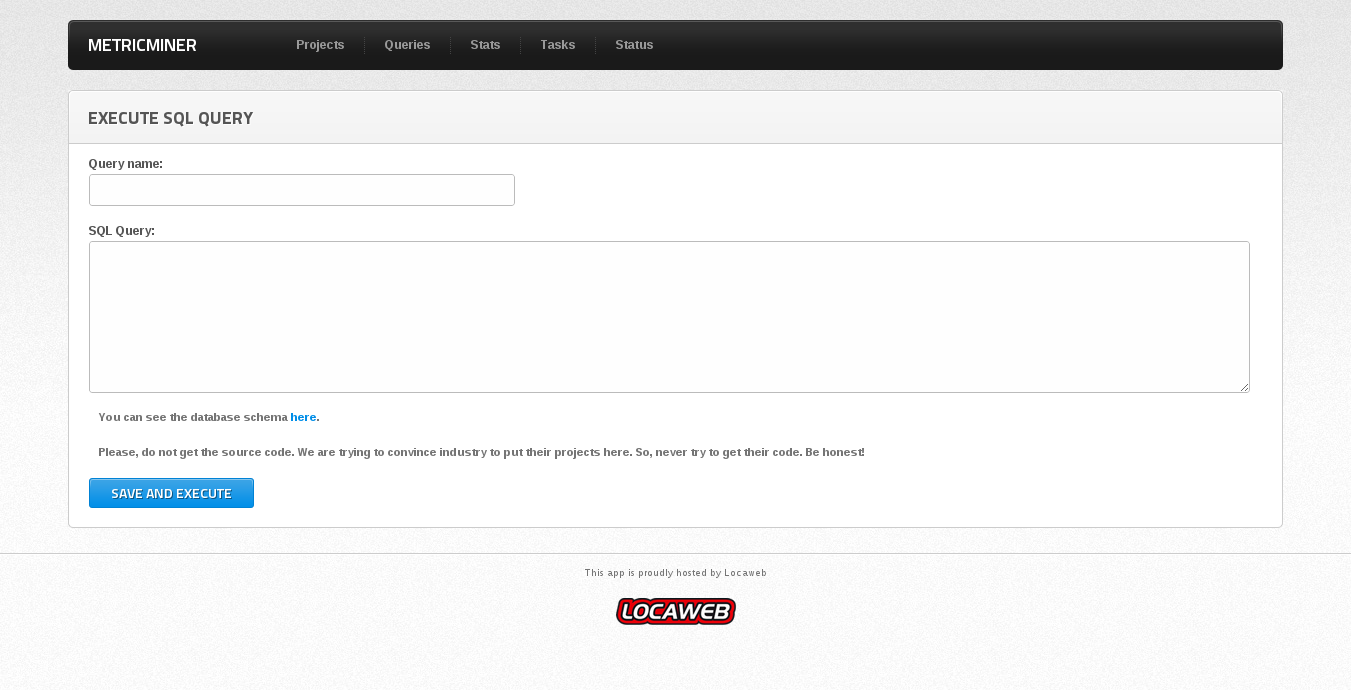
\includegraphics[width=1.00\textwidth]{img/query.png}
            \caption{Tela de consulta aos dados armazenados}
            \label{fig:screen_query}
        \end{figure}
        \clearpage

    \section{Tecnologias envolvidas} \label{sc:tecnologias}

        Nessa seção serão descritas brevemente as tecnologias envolvidas no desenvolvimento do MetricMiner.

        \subsection*{VRaptor 3}
            O VRaptor\footnote{\url{http://vraptor.caelum.com.br/}} é um \textit{framework} para desenvolvimento 
            web em java. Este \textit{framework} foca na simplicidade e no padrão de convenção sobre 
            configuração\footnote{\url{http://en.wikipedia.org/wiki/Convention_over_configuration}} para tornar o 
            desenvolvimento mais simples e eficiente. O VRaptor também se baseia fortemente no conceito de injeção 
            de dependências \cite{fowlerdi}. A ideia por trás deste padrão é que as dependências de uma classe 
            são criadas pelo container e não pela aplicação que utiliza tais dependências. O MetricMiner utiliza a 
            injeção de dependências em diversos componentes importantes da arquitetura que serão descritos com 
            mais detalhes na seção \ref{sc:arquitetura}

        \subsection*{Hibernate}
            O Hibernate é uma biblioteca de mapeamento objeto-relacional. Utilizando essa biblioteca, é possível 
            mapear classes do sistema a tabelas de um banco de dados relacional de forma transparente para o 
            desenvolvedor. Ou seja, é possível persistir e recuperar os dados sem que seja necessário escrever 
            queries SQL explicitamente. Para minimizar a  quantidade de requisições ao banco de dados, o Hibernate 
            faz cache em memória dos dados que serão persistidos. Em alguns pontos do MetricMiner esse 
            comportamento padrão do Hibernate teve que ser modificado, já que diversas tarefas realizadas no 
            sistema manipulam um volume grande de dados, o que acabou consumindo muita memória na máquina virtual 
            do Java.

        \subsection*{HTML, CSS e JavaScript}
            O MetricMiner é uma aplicação web, portanto a interface com o usuário foi desenvolvida em HTML, CSS e Javascript, que são linguagens interpretadas por um navegador web. HTML (\textit{HyperText Markup Language}) é uma linguagem de marcação, utilizada para estruturar uma página renderizada pelo navegador. CSS (\textit{Cascading Style Sheets}) é uma linguagem declarativa utilizada especificar o layout dos elementos representados em HTML. JavaScript é uma linguagem de script executada pelo navegador após o carregamento da página, por meio dessa linguagem é possível criar efeitos na página renderizada pelo navegador, criando interfaces mais ricas. Como o foco deste trabalho não é no desenvolvimento da interface, foi utilizado um template de HTML e CSS com o layout básico das páginas do sistema. Para a exibição dos gráficos dos projetos foi utilizada a biblioteca em JavaScript \textit{Google Chart Tools}\footnote{https://developers.google.com/chart/}.



    \section{Decisões arquiteturais} \label{sc:arquitetura}
    (revisar)
    %   eu colocaria aqui um paragrafo inicial descrevendo em alto nivel o sistema…
    %   web java deployado em um tomcat, que usa mysql como base de dados, processamento assincrono para execucao 
    %   de  jobs.. talvez ate um diagrama de componentes para exemplificar

        \subsection*{Modelo de dados}
            O diagrama da Figura \ref{fig:uml_modelo} exibe as principais classes do modelo de dados minerados pelo MetricMiner. Todas as classes e relacionamentos representados nesse diagrama são mapeados em tabelas no banco de dados por meio do Hibernate. 

                % use estereotipos. tipo Project <<contém>> artefatos pra facilitar a leitura
                % Kd a interface comum entre os Result? Se não existe, puxar uma nota ou coisa do tipo pra explicar
                \begin{figure}[ht]
                    \centering
                    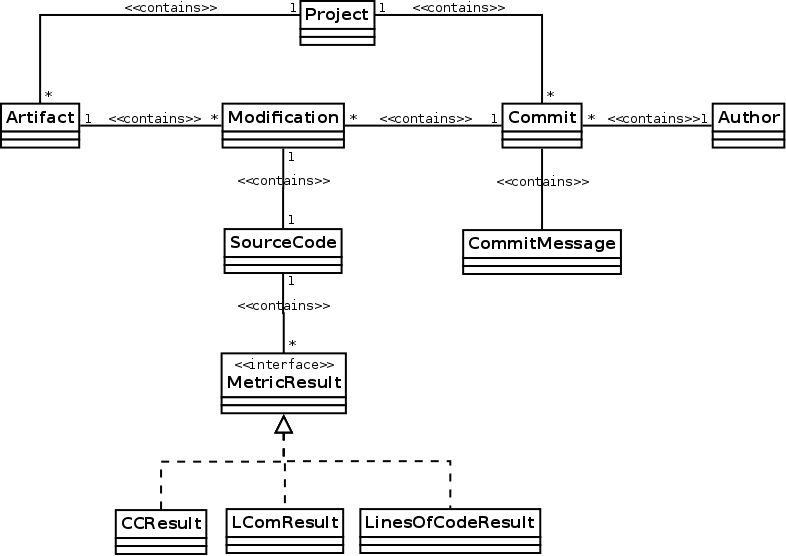
\includegraphics[width=1.00\textwidth]{img/uml-modelo.png}
                    \caption{Classes do modelo de dados}
                    \label{fig:uml_modelo}
                \end{figure}

            Com esse modelo, todo o histórico do sistema de controle de versão de um projeto fica armazenado no sistema. Cada \textit{commit} está relacionado ao conjunto de modificações realizadas nesse \textit{commit}. Uma modificação pode ser de três tipos: modificação comum, adição ou remoção. Adição ou remoção representam que o artefato foi adicionado ou removido do versionamento. Se o artefato não for binário, a modificação fica associada ao texto deste artefato (armazenado na classe \codechunk{SourceCode}). Dessa forma, todos as versões de cada arquivo de código do projeto ficam armazenados na base de dados. Cada versão dos arquivos de código fica associada ao resultado da execução de diferentes métricas. Para simplificar o diagrama, foram representadas apenas as classes \codechunk{CCResult}, \codechunk{LCOMResult} e \codechunk{LinesOfCodeResult} que armazenam os resultados das métricas de código complexidade ciclomática, LCOM e número de linhas de código, respectivamente. Existem outras quatro classes que armazenam resultados de outras métricas.

        \subsection*{Fila de execução} %% TaskRunner, RunnableTask, RunnableTaskFactory,
            Existem diferentes tipos de tarefas que são executadas no MetricMiner, por exemplo clonar um repositório de código, processar informações do sistema de controle de versão, entre outras. Para cada tipo de tarefa, existem duas classes associadas que implementam duas interfaces. A primeira é a 
            \codechunk{RunnableTask}, essa interface define apenas um método, \codechunk{run}, que deve executar o trabalho dessa tarefa. A segunda é a \codechunk{RunnableTaskFactory} onde está definido o método \codechunk{build}, que devolve uma instância de uma \codechunk{RunnableTask} para ser executada sobre um projeto específico. Essa é uma aplicação do padrão de projeto \codechunk{Abstract Factory} \cite{gof} e permitiu desacoplar os objetos que executam o trabalho da tarefa da construção desses objetos. O diagrama na Figura \ref{fig:uml_runner} exibe as classes que representam as principais tarefas executadas no MetricMiner.

            \begin{figure}[ht]
                \centering
                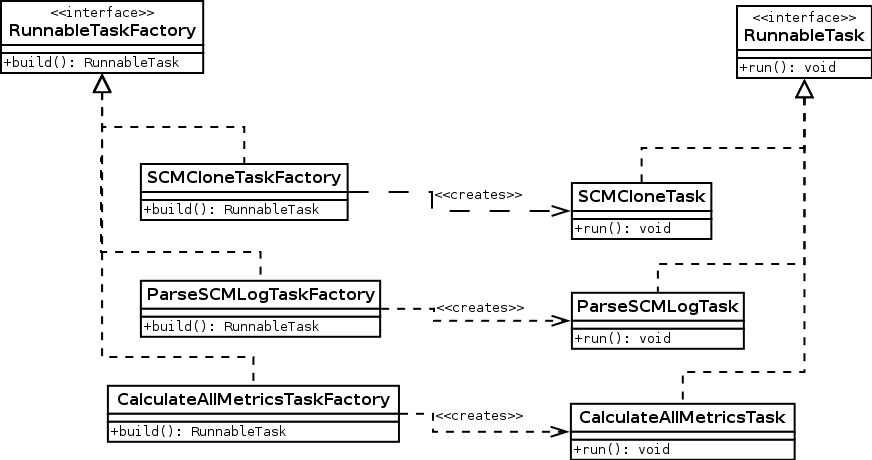
\includegraphics[width=1.00\textwidth]{img/uml-runner.png}
                \caption{Diagrama das classes que executam as tarefas do MetricMiner}
                \label{fig:uml_runner}
            \end{figure}

            Para inserir uma tarefa na fila, as informações dessa são inseridas no banco de dados, incluindo o nome completo (\textit{Fully qualified name}) da classe que implementa \codechunk{RunnableTaskFactory} dessa tarefa em particular. Depois, o método \codechunk{execute} da classe \codechunk{TaskRunner} extrai essas informações e constrói uma instância da factory dessa tarefa por meio da 
            \textit{Reflection API}\footnote{\url{http://docs.oracle.com/javase/tutorial/reflect/index.html}} do Java. Finalmente, uma intância de \codechunk{RunnableTask} é construída e executada. Esse método é executado a cada dez segundos e caso nenhuma tarefa esteja sendo executada, ela realiza o processo descrito anteriormente. Para a implementação da classe \codechunk{TaskRunner}, foi utilizado o plugin vraptor-tasks\footnote{\url{https://github.com/wpivotto/vraptor-tasks}}, que utiliza o  quartz, um famoso \textit{framework} para escalonamento de tarefas no mundo java.

            Dessa forma, desenvolver novas tarefas é simples, basta criar duas classes implementando as interfaces descritas anteriormente e tal tarefa já poderá ser inserida a fila de execução do MetricMiner por meio do banco de dados.

        \subsection*{Cálculo das métricas de código} %% Metric, MetricFactory, CalculateAllMetricsTask (template method), CalculateMetricTask

            % diagrama uml aqui, mesmo que simples, cai bem :)
            % comentar das metricas que sao executadas depois de todas as do repositorio. 
            % Como vc chamou isso mesmo?
            % comentar que usamos o japaparser aqui, que eh baseado no ANTLR (confirmar no site) para parsear 
            % codigo java. isso facilita a vida. 
            % mostrar como funciona isso, abre qquer visitor, e veja como eh, e detalha! 
            De forma semelhante à arquitetura das tarefas da fila execução, também foi utilizado o padrão \codechunk{Abstract Factory} no design das métricas de código implementadas no MetricMiner. Assim, para cada métrica, existem duas classes implementando duas interfaces: \codechunk{Metric} e \codechunk{MetricFactory}. A interface \codechunk{MetricFactory} define apenas um método, \codechunk{build}, que devolve uma instância da métrica. A interface \codechunk{Metric} define dois métodos principais: 

            \begin{itemize}
                \item \codechunk{void calculate(InputStream input)}: calcula a métrica para o código forncecido no \codechunk{InputStream}.
                \item \codechunk{Collection<MetricResult> results()}: devolve uma coleção de objetos que representam os resultados dessa métrica que serão armazenados no banco de dados.
            \end{itemize}

            Para encontrar as classes que implementam as métricas no classpath do MetricMiner, foi utilizado o recurso de \textit{Annotations}\footnote{\url{http://docs.oracle.com/javase/tutorial/java/javaOO/annotations.html}} do Java. Todas as classes que implementam métricas são anotadas com a anotação \codechunk{@MetricComponent}. Na inicialização do sistema, a classe \codechunk{MetricMinerConfigs} encontra todas as classes anotadas e as adiciona a lista de métricas registradas.

            Para executar tais métricas, a classe \codechunk{CalculateAllMetricsTask} é executada na fila de execução. Essa tarefa recebe as métricas registradas, percorre todas as versões de código de um determinado projeto cadastrado calculando todas as métricas e persistindo os resultados. De forma semelhante, a tarefa \codechunk{CalculateMetricTask} cálcula uma métrica específica para todas as versões de um projeto. 

            % falar tb da parte de SCM, como funciona a interface SCM. explicar os métodos da interface e como  
            % fazer para suportar novos.
            % fala do MVC tb. como o vraptor implementa MVC, onde ficam os controllers, como funciona uma 
            % requisição.

    \section{Estendendo e contribuindo com o projeto}

    %% nova métrica, nova métrica pós processamento, novos scv (svn já foi), novas tasks em geral (minerar listas de email, )
    
\chapter{Avaliação da ferramenta} \label{ch:avaliacao}

    \section{Resultados obtidos com a mineração de repositórios públicos}

    \section{Estudo de caso}

\chapter{Conclusão e trabalhos futuros} \label{ch:conclusao}

\chapter{Parte subjetiva} \label{ch:subjetiva}

\bibliographystyle{sbc}
\bibliography{monografia}

\end{document}


